% Template for PLoS
% Version 3.4 January 2017
\documentclass[10pt,letterpaper]{article}
\usepackage[top=0.85in,left=2.75in,footskip=0.75in]{geometry}

% amsmath and amssymb packages, useful for mathematical formulas and symbols
\usepackage{amsmath,amssymb}

% Use adjustwidth environment to exceed column width (see example table in text)
\usepackage{changepage}

% Use Unicode characters when possible
\usepackage[utf8x]{inputenc}

% textcomp package and marvosym package for additional characters
\usepackage{textcomp,marvosym}

% cite package, to clean up citations in the main text. Do not remove.
% \usepackage{cite}

% Use nameref to cite supporting information files (see Supporting Information section for more info)
\usepackage{nameref,hyperref}

% line numbers
\usepackage[right]{lineno}

% ligatures disabled
\usepackage{microtype}
\DisableLigatures[f]{encoding = *, family = * }

% color can be used to apply background shading to table cells only
\usepackage[table]{xcolor}

% array package and thick rules for tables
\usepackage{array}

% create "+" rule type for thick vertical lines
\newcolumntype{+}{!{\vrule width 2pt}}

% create \thickcline for thick horizontal lines of variable length
\newlength\savedwidth
\newcommand\thickcline[1]{%
  \noalign{\global\savedwidth\arrayrulewidth\global\arrayrulewidth 2pt}%
  \cline{#1}%
  \noalign{\vskip\arrayrulewidth}%
  \noalign{\global\arrayrulewidth\savedwidth}%
}

% \thickhline command for thick horizontal lines that span the table
\newcommand\thickhline{\noalign{\global\savedwidth\arrayrulewidth\global\arrayrulewidth 2pt}%
\hline
\noalign{\global\arrayrulewidth\savedwidth}}


% Remove comment for double spacing
%\usepackage{setspace} 
%\doublespacing

% Text layout
\raggedright
\setlength{\parindent}{0.5cm}
\textwidth 5.25in 
\textheight 8.75in

% Bold the 'Figure #' in the caption and separate it from the title/caption with a period
% Captions will be left justified
\usepackage[aboveskip=1pt,labelfont=bf,labelsep=period,justification=raggedright,singlelinecheck=off]{caption}
\renewcommand{\figurename}{Fig}

% Use the PLoS provided BiBTeX style
% \bibliographystyle{plos2015}

% Remove brackets from numbering in List of References
\makeatletter
\renewcommand{\@biblabel}[1]{\quad#1.}
\makeatother

% Leave date blank
\date{}

% Header and Footer with logo
\usepackage{lastpage,fancyhdr,graphicx}
\usepackage{epstopdf}
\pagestyle{myheadings}
\pagestyle{fancy}
\fancyhf{}
\setlength{\headheight}{27.023pt}
\lhead{
\includegraphics[width=2.0in]{PLOS-submission.eps}}
\rfoot{\thepage/\pageref{LastPage}}
\renewcommand{\footrule}{\hrule height 2pt \vspace{2mm}}
\fancyheadoffset[L]{2.25in}
\fancyfootoffset[L]{2.25in}
\lfoot{\sf PLOS}

%% Include all macros below
\newcommand{\lorem}{{\bf LOREM}}
\newcommand{\ipsum}{{\bf IPSUM}}

\usepackage{color}
\usepackage{fancyvrb}
\newcommand{\VerbBar}{|}
\newcommand{\VERB}{\Verb[commandchars=\\\{\}]}
\DefineVerbatimEnvironment{Highlighting}{Verbatim}{commandchars=\\\{\}}
% Add ',fontsize=\small' for more characters per line
\usepackage{framed}
\definecolor{shadecolor}{RGB}{248,248,248}
\newenvironment{Shaded}{\begin{snugshade}}{\end{snugshade}}
\newcommand{\KeywordTok}[1]{\textcolor[rgb]{0.13,0.29,0.53}{\textbf{#1}}}
\newcommand{\DataTypeTok}[1]{\textcolor[rgb]{0.13,0.29,0.53}{#1}}
\newcommand{\DecValTok}[1]{\textcolor[rgb]{0.00,0.00,0.81}{#1}}
\newcommand{\BaseNTok}[1]{\textcolor[rgb]{0.00,0.00,0.81}{#1}}
\newcommand{\FloatTok}[1]{\textcolor[rgb]{0.00,0.00,0.81}{#1}}
\newcommand{\ConstantTok}[1]{\textcolor[rgb]{0.00,0.00,0.00}{#1}}
\newcommand{\CharTok}[1]{\textcolor[rgb]{0.31,0.60,0.02}{#1}}
\newcommand{\SpecialCharTok}[1]{\textcolor[rgb]{0.00,0.00,0.00}{#1}}
\newcommand{\StringTok}[1]{\textcolor[rgb]{0.31,0.60,0.02}{#1}}
\newcommand{\VerbatimStringTok}[1]{\textcolor[rgb]{0.31,0.60,0.02}{#1}}
\newcommand{\SpecialStringTok}[1]{\textcolor[rgb]{0.31,0.60,0.02}{#1}}
\newcommand{\ImportTok}[1]{#1}
\newcommand{\CommentTok}[1]{\textcolor[rgb]{0.56,0.35,0.01}{\textit{#1}}}
\newcommand{\DocumentationTok}[1]{\textcolor[rgb]{0.56,0.35,0.01}{\textbf{\textit{#1}}}}
\newcommand{\AnnotationTok}[1]{\textcolor[rgb]{0.56,0.35,0.01}{\textbf{\textit{#1}}}}
\newcommand{\CommentVarTok}[1]{\textcolor[rgb]{0.56,0.35,0.01}{\textbf{\textit{#1}}}}
\newcommand{\OtherTok}[1]{\textcolor[rgb]{0.56,0.35,0.01}{#1}}
\newcommand{\FunctionTok}[1]{\textcolor[rgb]{0.00,0.00,0.00}{#1}}
\newcommand{\VariableTok}[1]{\textcolor[rgb]{0.00,0.00,0.00}{#1}}
\newcommand{\ControlFlowTok}[1]{\textcolor[rgb]{0.13,0.29,0.53}{\textbf{#1}}}
\newcommand{\OperatorTok}[1]{\textcolor[rgb]{0.81,0.36,0.00}{\textbf{#1}}}
\newcommand{\BuiltInTok}[1]{#1}
\newcommand{\ExtensionTok}[1]{#1}
\newcommand{\PreprocessorTok}[1]{\textcolor[rgb]{0.56,0.35,0.01}{\textit{#1}}}
\newcommand{\AttributeTok}[1]{\textcolor[rgb]{0.77,0.63,0.00}{#1}}
\newcommand{\RegionMarkerTok}[1]{#1}
\newcommand{\InformationTok}[1]{\textcolor[rgb]{0.56,0.35,0.01}{\textbf{\textit{#1}}}}
\newcommand{\WarningTok}[1]{\textcolor[rgb]{0.56,0.35,0.01}{\textbf{\textit{#1}}}}
\newcommand{\AlertTok}[1]{\textcolor[rgb]{0.94,0.16,0.16}{#1}}
\newcommand{\ErrorTok}[1]{\textcolor[rgb]{0.64,0.00,0.00}{\textbf{#1}}}
\newcommand{\NormalTok}[1]{#1}




\usepackage{forarray}
\usepackage{xstring}
\newcommand{\getIndex}[2]{
  \ForEach{,}{\IfEq{#1}{\thislevelitem}{\number\thislevelcount\ExitForEach}{}}{#2}
}

\setcounter{secnumdepth}{0}

\newcommand{\getAff}[1]{
  \getIndex{#1}{Smith College}
}

\providecommand{\tightlist}{%
  \setlength{\itemsep}{0pt}\setlength{\parskip}{0pt}}

\begin{document}
\vspace*{0.2in}

% Title must be 250 characters or less.
\begin{flushleft}
{\Large
\textbf\newline{Classification of Wildtype and Mutant Zebrafish Brains via Computational
Method} % Please use "sentence case" for title and headings (capitalize only the first word in a title (or heading), the first word in a subtitle (or subheading), and any proper nouns).
}
\newline
\\
Shuli Hu\textsuperscript{\getAff{Smith College}},
Wencong Li\textsuperscript{\getAff{Smith College}},
Dejia Tang\textsuperscript{\getAff{Smith College}},
Ji Young Yun\textsuperscript{\getAff{Smith College}}\\
\bigskip
\textbf{\getAff{Smith College}}Statistical and Data Sciences, Northampton, MA\\
\bigskip
\end{flushleft}
% Please keep the abstract below 300 words
\section*{Abstract}
Classification of biological creatures' phenotypes has long been a field
that scientists study at. In this project, we utilize support vector
machine to distinguish structures of Zebrafish's brains by using data
generated from landmark analysis (cited Morgan's paper). We create a
tool for biologists to intuitively classify three-dimensional biological
shapes into two groups, usually defined as wild type and mutant, and
understand which part of the shapes have the most impact on the
classification result. This project derives from Professor Barresi's
biological image analysis research at Smith College.

% Please keep the Author Summary between 150 and 200 words
% Use first person. PLOS ONE authors please skip this step. 
% Author Summary not valid for PLOS ONE submissions.   

\linenumbers

% Use "Eq" instead of "Equation" for equation citations.
\section{Acknowledgements}\label{acknowledgements}

This project was completed in partial fulfillment of the requirements of
SDS 410: SDS Capstone. This course is offered by the Statistical and
Data Sciences Program at Smith College, and was taught by Benjamin
Baumer in Spring 2018.

\section{Introduction}\label{introduction}

This project derives from Professor Barresi's biological image analysis
research at Smith College and provides a tool to classify the structures
within zebrafish brains via support vector machine. Our goal is to
distinguish the wild and mutant types of zebrafish brain's structures.
Morgan, a student in Barresi Lab, used landmarks analysis to divide the
points in the three-dimentional images into small wedges and computed
the landmark, which is the most representative point, within each wedge.
The image of signals in a Zebrafish brain is shown in Figure 1. The
shape is divided into 30 slices, and each slice is further divided into
8 wedges. The landmark in each wedge is calculated by taking the median
distance of all points in each wedge, \(R\). We use number of points in
each wedge and median R to run SVM models to do classifications.

\subsection{Landmark Analysis}\label{landmark-analysis}

\subsection{Programming languages
used}\label{programming-languages-used}

\subsubsection{Python}\label{python}

\subsubsection{R}\label{r}

\subsubsection{Git}\label{git}

\section{Literature Review}\label{literature-review}

Research in developmental biology has relied on the analysis of
morphological phenotypes through qualitative examination of maximum
intensity projections that surrender the power of three dimensional
data. Statistical methods to analyze visual data are needed,
particularly to detect subtle phenotypes.

Morgan et al. (2018) have utilized the open source program, Ilastik,
which employs a training based machine learning, to eliminate the image
noise. Then they preformed principal component analysis to align
commissures between samples, reducing misalignment artifacts, and
implemented a cylindrical coordinate system which preserves image
dimensionality normally lost in maximum intensity projection (MIP),
which facilitates presentation of the data, but sacrifices much of the
complexity and relational data contained in the image. Then they reduced
the points identified by the program as belonging to the structure to a
set of landmark points that describe the shape and distribution of
signal corresponding to the structure. Finally, using the landmark
system, we are able to identify and quantify structural differences and
changes in signal distribution between wild type and mutant commissures.

Landmarks describe a shape by locating a finite number of points on each
specimen. There are three basic types of landmarks: scientific,
mathematic and pseudo-landmarks. A scientific landmark is a point
assigned by an expert that corresponds between objects in some
scientifically meaningful way, for example the corner of an eye.
Mathematical landmarks are points located on an object according to some
mathematical or geometrical property of the figure. Since it does not
assume a preference of one location to another, it is particularly
useful in automated morphological recognition and analysis for
under-studied structure. Pseudo-landmarks are constructed points on an
object, located either around the outline or in between scientific or
mathematic landmarks. It is often used to approximate continuous curves
(Dryden and Mardia, 2016). This research has chosen to calculate an
automatic set of landmarks distributed across the structure in order to
avoid introducing bias due to expectations about where biological
differences should emerge.

Morgan et al. used Random Forest machine leaning method to classify the
landmarks. Although the classification is quite accurate, it is
difficult to interpret the result from biological aspects. Instead of
doing classification on all of the landmarks at the same time, we
decided to do classifacation on one landmark at a time via Support
Vector Machine. The SVM algorithm is a classification algorithm that
provides state-of-the-art performance in a wide variety of application
domains, image classification. During the past few years, SVM has been
applied very broadly within the field of computational biology
especially in pattern recognition problems, including protein remote
homology detection, microarray gene expressions analysis, prediction of
protein-protein interactions, etc.

In 1999, Jaakkola et al. ushered in stage 4 of the development of
homology detection algorithms with a paper that garnered the ``Best
paper'' award at the annual Intelligent Systems for Molecular Biology
conference. Their primary insight was that additional accuracy can be
obtained by modeling the difference between positive and negative
examples. Because the homology task required discriminating between
related and unrelated sequences, explicitly modeling the difference
between these two sets of sequences yields an extremely powerful method.

\section{Data and Variables}\label{data-and-variables}

We have 43 wildtypes samples and 35 mutant samples for training and
testing. There are 152 landmarks for each sample, with each of them
containing the following variables: number of points in that wedge
median R (micro-meter): the median of the distances to the center of the
slice of all the points in that wedge. alpha (micro-meter): distance
from the center of the landmark to the midline theta (radian): the
degree that shows the location of the wedge of a slice

We used the number of points and the median R to do classification via
support vector machine. For missing `median R' values due to absence of
points in particular landmarks, we filled them with the median value of
all the points in that landmark.

\subsection{Tidy Data}\label{tidy-data}

The original landmarks data is a wide table containing the sample index
and all the columns holding information regarding the minimum and
maximum values of Alpha and Theta, number of points, median r value, and
the type of sample for a particular sample in each landmark. However,
because all of such variables were joined by underscores in the variable
names, such as \texttt{-14.29\_-4.76\_-0.79\_0.0\_50\_pts} or
\texttt{-14.29\_-4.76\_-0.79\_0.0\_50\_r} and the value in each cell
refers to the median r value or number of points, it was very difficult
to see what each column actually represented. The ideal format of the
data set was to have the sample index, minimum and maximum Alpha,
minimum and maximum Theta, number of points, median r, and type of
sample each be its own column. Hence, three key functions were used from
the tidyr package: gather, separate, and spread. The gather function
separated the dataset into key and value pairs for each index. The key
was the column name containing all essential information connected by
underscores and the value included the number of points or median r
value. Then, the separate function separated the result from the gather
function divided the column connected by underscore into 5 different
columns, named as \texttt{min\_alpha}, \texttt{max\_alpha},
\texttt{min\_theta}, \texttt{max\_theta}, and \texttt{ptsOrR}. This was
added to the result of the gather function that contained the index and
value of each cell, either median R or number of points. Afterwards, the
spread function widened the already wide table by expanding the
\texttt{ptsOrR} column by creating two columns, each column representing
median R and the number of points.

\subsection{Dealing with Missing
Value}\label{dealing-with-missing-value}

Samples with missing values are eliminated by Supporting vector machine.
For wedges that do not have any point in it, \texttt{median\ r} cannot
be calculated, which means that these sample will be eliminated when
running SVM. Wedges without points have biologically meanings, and we
should not ignore these wedges in our model. In order to keep the wedges
in our model, we need to artificially pick a \texttt{median\ r} value to
replace the missing ones. Supporting vector machine is sensitive to
outliers, so we cannot pick an \texttt{r} value that could become
outliers. We decided to calculate the mean of \texttt{median\ r} for the
nth landmark of all 78 samples, and then we replace the missing
\texttt{median\ r} values with the mean.

\section{Supporting Vector Machine}\label{supporting-vector-machine}

SVM's have been proven to be a powerful algorithm for supervised
clustering. During the past few years, SVM has been applied very broadly
within the field of computational biology especially in pattern
recognition problems. The goal of SVM is to find a seperation line
\(f(x) = (\beta_0 + \beta_1 * x_1 + \beta_2 * x_2)\) that separates the
nearest data as clean as possible. The parameters \(\beta\) are found by
solving the optimization problem --to maximize M subject to some
restrictions -- in 2 dimensions below.

\begin{itemize}
\tightlist
\item
  \(C\): tuning parameter, toleration of violation.
\item
  \(M\): margin, distance of the closest points to the hyperplane.
\item
  \(e_i\) : slack variable, correct/incorrect classification of a point.
\end{itemize}

The function of the seperation line:

\[f(x) = \beta_0 + \beta_1 * x_1 + \beta_2 * x_2 \]

if \(f(x) = 0\), the observation is on the seperation line.

\[ y * ( \beta_0 + \beta_1 * x_1 + \beta_2 * x_2 )\] is the
perpendicular distance from the ith observation to the hyperplane. If
it's \textgreater{}0, the observation falls at the right side of the
speration line and vice versa.

\section{Workflow and User Interface}\label{workflow-and-user-interface}

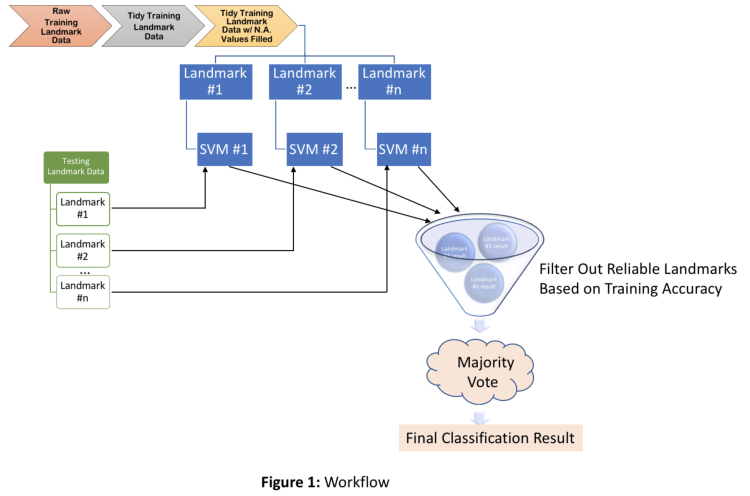
\includegraphics{zebrafish_paper_files/figure-latex/unnamed-chunk-1-1.pdf}

\subsection{Step One: Data Processing and
Modelling}\label{step-one-data-processing-and-modelling}

This step is implemented using Python and packages including pandas,
nump and sklearn are required. Users would need to run and interact with
the Python script \texttt{svm.py} to build the model and pre-process the
data if needed.

The script \texttt{svm.py} contains two components: a general-purpose
\texttt{svm\_classification()} function that builds a SVM model to
classify points for a perticular landmark and a \texttt{main()} function
that runs the \texttt{svm\_classification()} function for each landmark.

\subsubsection{User Interaction}\label{user-interaction}

\subsubsection{Input File}\label{input-file}

Input file must contain landmark data. Variables that are needed for
classification are required to be included in the input file. In our
analysis, we used number of points in each sub-section corresponding to
each landmark of the 3D shape and the \texttt{median\ R} of points in
each wedge.

\subsubsection{Sample input file}\label{sample-input-file}

\subsubsection{Output File}\label{output-file}

\subsection{Step Two: Result Analyzation and
Visualization}\label{step-two-result-analyzation-and-visualization}

\subsection{Testing}\label{testing}

\subsubsection{Cross-Validation}\label{cross-validation}

For our project, we have access to 43 wild-type samples and 35
mutant-type samples. Due to this limited sample size, we dicided to use
a leave-one-out cross validation method to test our model.\\
For each testing sample, we built 152 SVMs for each landmark. For each
SVM, we used 10-fold cross validation to select a tuning parameter C
value among 0.1, 1 and 10. After we get precision scores and predictions
of each landmark, we will present the distribution of the landmarks'
precision scores (Figure 3). The user would then be allowed to set a
threshold for certain precision scores to select out a subset of
landmarks that are considered significant. A majority vote would then be
performed among the selected landmarks to get an overall prediction for
the sample.

\section{Result}\label{result}

\subsection{Visulization}\label{visulization}

\section{Discussion}\label{discussion}

\subsection{Strengths}\label{strengths}

The SVM model application on landmark data gives insightful analysis of:
which landmark (=which part of the brain) carries more information of
the type. whether a new sample is of mutant or wild type

In the previous method random forest, the number of predictors p exceeds
the number of samples. Morgan applied PCA do reduce the dimension of the
predictors. The problem with dimension reduction is that it gives a
linear combination of the dimensions that are projected on those are
kept. While the largest projections still make sense, the minor
projections are very random and thus difficult to interpret.

\subsection{Limitations}\label{limitations}

The SVM model also has its limitation in that it only considers one
single landmark at a time without considering the relationship across
the landmarks of the whole sample.

\subsection{Improvements}\label{improvements}

Itenerating machine learning

Instead of cross-validation, better results could be achieved by using
itenerating machine learning method. In iterative machine learning we
repeat the process of training and testing several times. At the first
round the user gives examples of objects belonging to some classes and
the machine learning algorithm is trained with this data. In the second
round, the algorithm shows examples of objects it thinks that belong to
these classes. Now, the user merely adds objects to the improved
training set which the machine learning algorithm has put into a wrong
class. That is, the user only corrects the ``misunderstandings'' of the
algorithm. In this way we can concentrate on difficult examples of
objects that are hard to classify or are for some reason easily missed
by humans. Such objects may lie close to the decision boundaries or in
the periphery in the multidimensional feature space. This iterative
process is continued until the machine learning algorithm does not make
any mistakes or the classification results do not improve anymore. It
will improve our classification results and thus is likely to help make
better predictions for unknown type.

\subsection{Future Study}\label{future-study}

We will continue to work on: making the program more user friendly
running more tests to prove the accuracy of our model

\section{Appendix Code}\label{appendix-code}

\subsection{Support Vector Machine}\label{support-vector-machine}

\subsection{Shiny App}\label{shiny-app}

\begin{Shaded}
\begin{Highlighting}[]
\NormalTok{list_of_indices <-}\StringTok{ }\KeywordTok{c}\NormalTok{(index}\OperatorTok{$}\NormalTok{Index, }\StringTok{"AT"}\NormalTok{, }\StringTok{"ZRF"}\NormalTok{)}
\NormalTok{list_of_scores <-}\StringTok{ }\KeywordTok{c}\NormalTok{(}\StringTok{"precision"}\NormalTok{, }\StringTok{"recall"}\NormalTok{, }\StringTok{"f1"}\NormalTok{, }\StringTok{"w_precision"}\NormalTok{, }\StringTok{"w_recall"}\NormalTok{, }\StringTok{"w_f1"}\NormalTok{, }\StringTok{"m_precision"}\NormalTok{, }\StringTok{"m_recall"}\NormalTok{, }\StringTok{"m_f1"}\NormalTok{)}
\NormalTok{landmark_xy <-}\StringTok{ }\KeywordTok{fread}\NormalTok{(}\StringTok{"/Users/priscilla/Desktop/SDS Capstone/Zebrafish/analysis/landmark_xy.csv"}\NormalTok{)}
\NormalTok{list_of_channel <-}\StringTok{ }\KeywordTok{c}\NormalTok{(}\StringTok{"AT"}\NormalTok{, }\StringTok{"ZRF"}\NormalTok{)}

\CommentTok{# User Interface}
\NormalTok{ui <-}\StringTok{ }\KeywordTok{fluidPage}\NormalTok{(}
  \KeywordTok{titlePanel}\NormalTok{(}\DataTypeTok{title=}\KeywordTok{h4}\NormalTok{(}\StringTok{"Classification of Wildtype and Mutant Zebrafish Brains via Computational Method"}\NormalTok{, }
                      \DataTypeTok{align=}\StringTok{"center"}\NormalTok{)),}
  \KeywordTok{selectInput}\NormalTok{(}\StringTok{"channel"}\NormalTok{, }\StringTok{"Channel:"}\NormalTok{, list_of_channel),}
  \KeywordTok{selectInput}\NormalTok{(}\StringTok{"sampleindex"}\NormalTok{, }\StringTok{"Sample Index:"}\NormalTok{, list_of_indices),}
  \KeywordTok{selectInput}\NormalTok{(}\StringTok{"score"}\NormalTok{, }\StringTok{"Accuracy Measurement:"}\NormalTok{, list_of_scores),}
  \KeywordTok{mainPanel}\NormalTok{(}\KeywordTok{fluidRow}\NormalTok{(}
              \KeywordTok{splitLayout}\NormalTok{(}\DataTypeTok{cellWidths =} \KeywordTok{c}\NormalTok{(}\StringTok{"90%"}\NormalTok{, }\StringTok{"60%"}\NormalTok{), }\KeywordTok{plotOutput}\NormalTok{(}\StringTok{"plot1"}\NormalTok{), }\KeywordTok{plotOutput}\NormalTok{(}\StringTok{"plot2"}\NormalTok{))}
\NormalTok{            ))}
\NormalTok{)}

\CommentTok{# Server}
\NormalTok{server <-}\StringTok{ }\ControlFlowTok{function}\NormalTok{(input,output) \{}
\NormalTok{  dat <-}\StringTok{ }\KeywordTok{reactive}\NormalTok{(\{}
\NormalTok{    dir <-}\StringTok{ }\KeywordTok{paste0}\NormalTok{(wd, }\StringTok{"/analysis/r"}\NormalTok{, input}\OperatorTok{$}\NormalTok{sampleindex, }\StringTok{"_med_"}\NormalTok{, input}\OperatorTok{$}\NormalTok{channel, }\StringTok{"_result.csv"}\NormalTok{)}
\NormalTok{    test <-}\StringTok{ }\KeywordTok{fread}\NormalTok{(dir)}
\NormalTok{    test <-}\StringTok{ }\NormalTok{test }\OperatorTok
\StringTok{      }\KeywordTok{left_join}\NormalTok{(landmark_xy, }\DataTypeTok{by=}\StringTok{"landmark_index"}\NormalTok{)}
    \KeywordTok{print}\NormalTok{(test)}
\NormalTok{    test}
\NormalTok{  \})}
  
  \CommentTok{# Plot One}
\NormalTok{  output}\OperatorTok{$}\NormalTok{plot1 <-}\StringTok{ }\KeywordTok{renderPlot}\NormalTok{(\{}
\NormalTok{    p1 <-}\StringTok{ }\KeywordTok{ggplot}\NormalTok{(}\KeywordTok{dat}\NormalTok{(), }
                 \KeywordTok{aes}\NormalTok{(}\DataTypeTok{x =}\NormalTok{ y, }\DataTypeTok{y =}\NormalTok{ x)) }\OperatorTok{+}
\StringTok{      }\KeywordTok{geom_tile}\NormalTok{(}\KeywordTok{aes}\NormalTok{(}\DataTypeTok{fill =}\NormalTok{ input}\OperatorTok{$}\NormalTok{score)) }\OperatorTok{+}
\StringTok{      }\KeywordTok{xlab}\NormalTok{(}\StringTok{"Alpha"}\NormalTok{) }\OperatorTok{+}
\StringTok{      }\KeywordTok{ylab}\NormalTok{(}\StringTok{"Theta"}\NormalTok{) }\OperatorTok{+}
\StringTok{      }\KeywordTok{scale_x_continuous}\NormalTok{(}\DataTypeTok{limits =} \KeywordTok{c}\NormalTok{(}\DecValTok{1}\NormalTok{, }\DecValTok{19}\NormalTok{), }\DataTypeTok{breaks=}\KeywordTok{c}\NormalTok{(}\DecValTok{1}\NormalTok{, }\DecValTok{10}\NormalTok{, }\DecValTok{19}\NormalTok{), }\DataTypeTok{labels=}\KeywordTok{c}\NormalTok{(}\StringTok{"-90.51"}\NormalTok{, }\StringTok{"0"}\NormalTok{, }\StringTok{"90.51"}\NormalTok{)) }\OperatorTok{+}
\StringTok{      }\KeywordTok{scale_y_continuous}\NormalTok{(}\DataTypeTok{limits =} \KeywordTok{c}\NormalTok{(}\DecValTok{1}\NormalTok{, }\DecValTok{8}\NormalTok{), }\DataTypeTok{breaks=}\KeywordTok{c}\NormalTok{(}\DecValTok{1}\NormalTok{, }\FloatTok{4.5}\NormalTok{, }\DecValTok{8}\NormalTok{), }\DataTypeTok{labels=}\KeywordTok{c}\NormalTok{(}\StringTok{"-3.14"}\NormalTok{,}\StringTok{"0"}\NormalTok{,}\StringTok{"3.14"}\NormalTok{)) }\OperatorTok{+}
\StringTok{      }\KeywordTok{scale_fill_continuous}\NormalTok{(}\DataTypeTok{limits=}\KeywordTok{c}\NormalTok{(}\DecValTok{0}\NormalTok{, }\DecValTok{1}\NormalTok{), }\DataTypeTok{breaks=}\KeywordTok{seq}\NormalTok{(}\DecValTok{0}\NormalTok{,}\DecValTok{1}\NormalTok{,}\DataTypeTok{by=}\FloatTok{0.25}\NormalTok{)) }
\NormalTok{    p1}
\NormalTok{  \})}
  
  \CommentTok{# Plot Two}
\NormalTok{  output}\OperatorTok{$}\NormalTok{plot2 <-}\StringTok{ }\KeywordTok{renderPlot}\NormalTok{(\{}
\NormalTok{    p2 <-}\StringTok{ }\KeywordTok{qplot}\NormalTok{(input}\OperatorTok{$}\NormalTok{score, }\DataTypeTok{geom =} \StringTok{"histogram"}\NormalTok{) }\OperatorTok{+}
\StringTok{      }\KeywordTok{xlab}\NormalTok{(}\StringTok{"Precision"}\NormalTok{) }\OperatorTok{+}
\StringTok{      }\KeywordTok{ylab}\NormalTok{(}\StringTok{"Count"}\NormalTok{)  }
\NormalTok{    p2}
\NormalTok{  \})}
  
\NormalTok{\}}
\end{Highlighting}
\end{Shaded}

\section*{References}\label{references}
\addcontentsline{toc}{section}{References}

\nolinenumbers


\end{document}

